\chapter{ผลการปฏิบัติงาน}
\label{chapter:result}
จากการปฏิบัติงานสหกิจศึกษาที่ บริษัท วงใน มีเดีย จำกัด (สำนักงานใหญ่) ด้วยตำแหน่ง Software Engineer (Backend) เป็นระยะเวลา 6 เดือน ตั้ง 4 มิถุนายน พ.ศ.2562 จนถึง 29 พฤศจิกายน พ.ศ.2562 สามารถสรุปผลการปฏิบัติงานได้ดังนี้
	
\section{ผลการปฏิบัติงาน}
ฟังก์ชันหลักของระบบจัดการโฆษณาแบบจำกัดจำนวนการคลิกและการแสดงโฆษณา สามารถทำงานตามที่ออกแบบไว้ โดยสามารถจำกัดการแสดงผลโฆษณาด้วยจำนวนการคลิกของโฆษณา และสามารถสร้างอีเมลรายงานสถิติของโฆษณาตามที่ UX/UI ของ Squad เป็นผู้ออกแบบ ส่งไปยังลูกค้าได้โดยอัตโนมัติได้ และมีหน้าแอดมินสำหรับให้พนักงานที่เกี่ยวข้องเข้ามาใช้งานเซอร์วิส Ad Report ได้ ดังภาพที่ 4.1 

\begin{figure}[!h]
	\centering
	\subfigure[]{
		\label{Fig:adminui:list}
		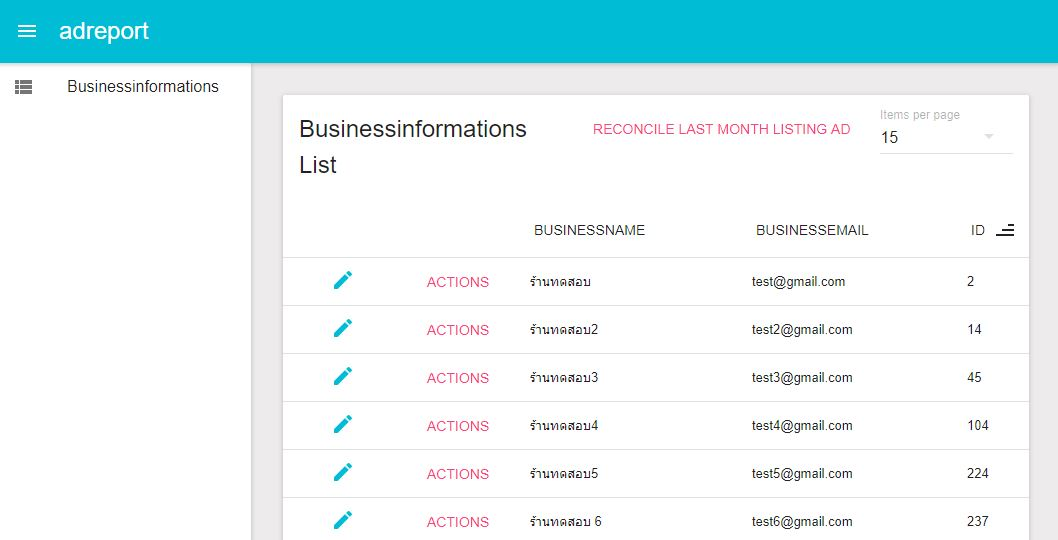
\includegraphics[width=0.85\textwidth]{admin-ui-1}  
	}
	\subfigure[]{
		\label{Fig:adminui:edit}
		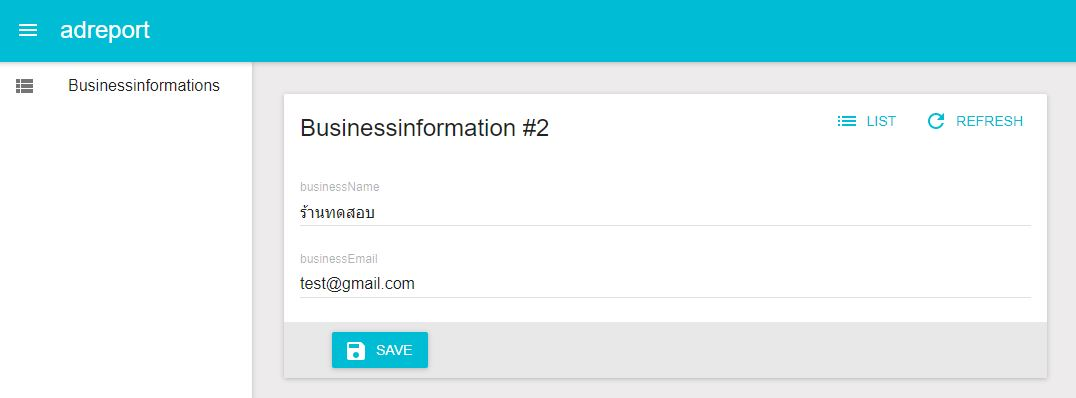
\includegraphics[width=0.85\textwidth]{admin-ui-2}  
	}
	\caption{หน้าแอดมินของเซอร์วิส Ad Report (ก) และหน้าแก้ไขข้อมูลต่าง ๆ ของร้าน (ข)}
	\label{Fig:adminui}
\end{figure}

โดยภายในหน้าแอดมินของเซอร์วิส Ad Report จะประกอบไปด้วยฟังก์ชันการทำงานต่าง ๆ ดังนี้

\begin{itemize}
	\item แก้ไขข้อมูลต่าง ๆ ของร้านได้โดยการกดไปที่ไอคอนดินสอสีฟ้า
	\item ส่งอีเมลรายงานสถิติของโฆษณารายสัปดาห์โดยการกดไปที่ปุ่ม ACTIONS สีแดง (สำหรับใช้งานในกรณีที่การส่งอัตโนมัติเกิดข้อผิดพลาด เจ้าหน้าที่คนอื่นจะสามารถส่งอีเมลรายงานด้วยตนเองได้) 
\end{itemize}

สำหรับรูปที่ 4.2 และ 4.3 จะเป็นตัวอย่างอีเมลรายงานผลการโฆษณาที่จะส่งไปยังอีเมลของลูกค้า ซึ่งจะมีรายงานที่เป็นไฟล์นามสกุล .pdf แนบในอีเมลด้วย โดยเนื้อหาภายในรายงานจะประกอบไปด้วยข้อมูลต่าง ๆ ได้แก่

\begin{itemize}
	\item ชื่อร้าน
	\item ช่วงเวลาของรายงาน
	\item จำนวนครั้งที่แสดงผลโฆษณาในช่วงเวลาของรายงาน
	\item จำนวนครั้งที่มีผู้ใช้คลิกเข้าไปที่โฆษณาในช่วงเวลาของรายงาน
	\item แผนภูมิแสดงจำนวนครั้งที่แสดงผลโฆษณาในช่วงเวลาของรายงานต่อวัน
	\item แผนภูมิแสดงจำนวนครั้งที่มีผู้ใช้คลิกเข้าไปที่โฆษณาในช่วงเวลาของรายงานต่อวัน
	\item จำนวนคลิกของโฆษณาที่ใช้ไปแล้ว
	\item จำนวนคลิกของโฆษณาคงเหลือ
\end{itemize}
	
\begin{figure}[!h]
	\centering
	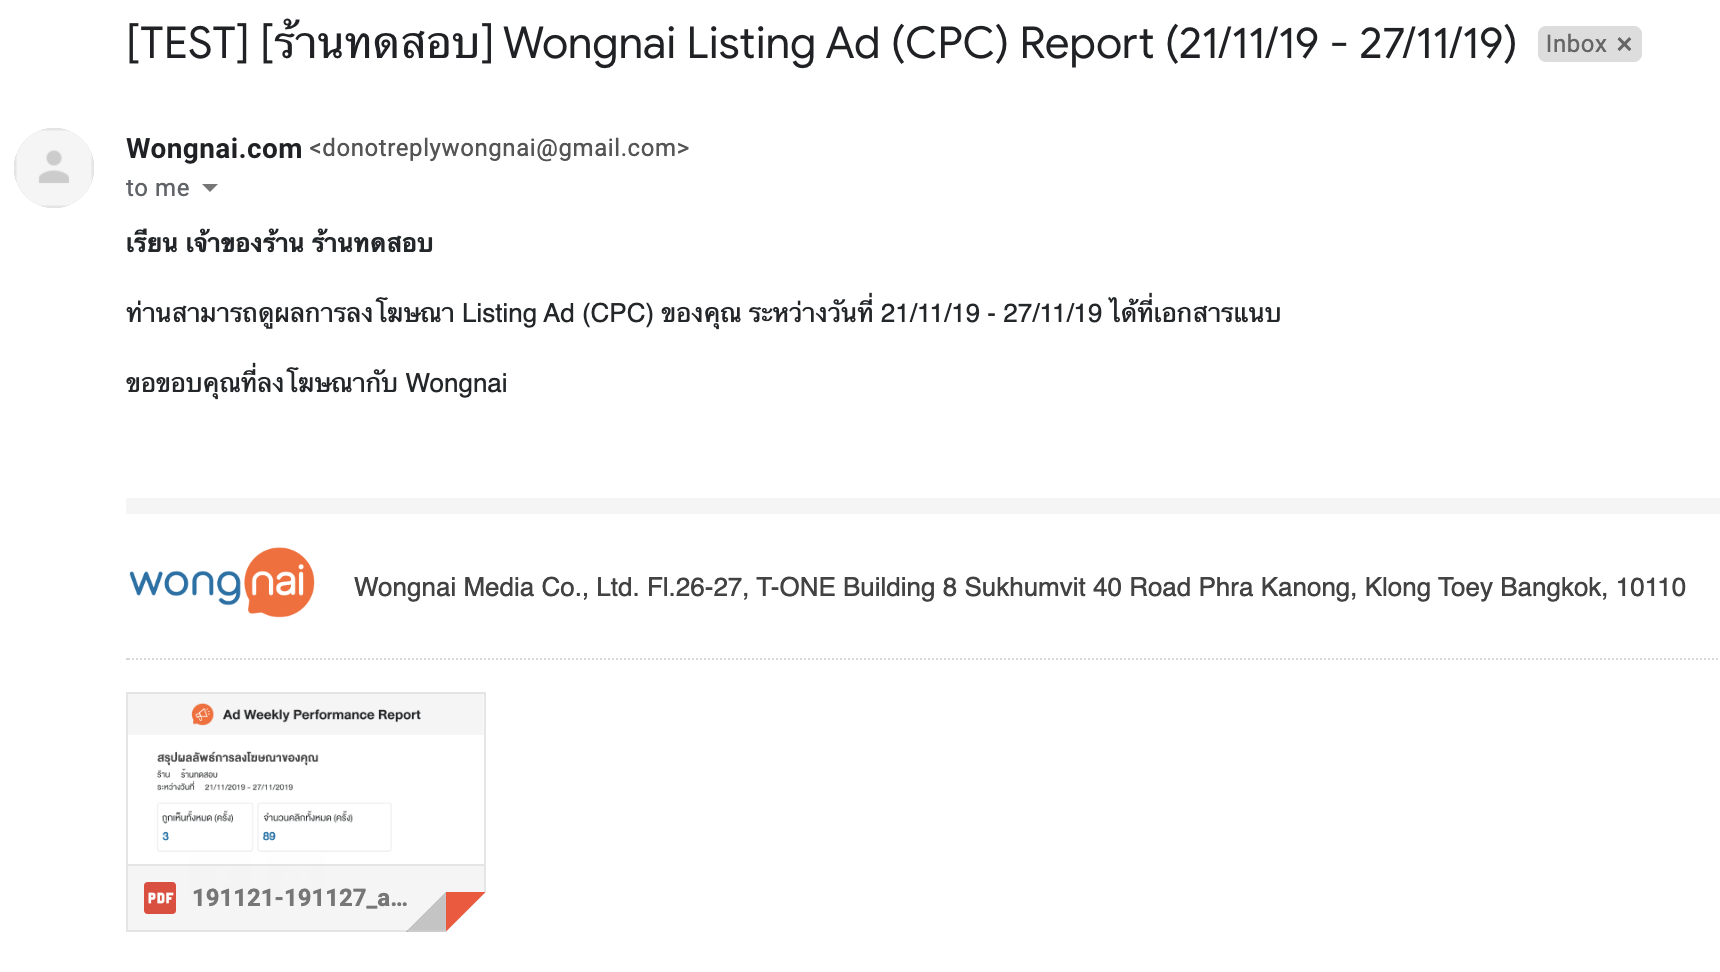
\includegraphics[width=1\textwidth]{report-email.png}  
	\caption{อีเมลรายงานสถิติของโฆษณาที่ส่งให้ลูกค้า}
	\label{Fig:report-email}
\end{figure}

\begin{figure}[!p]
	\centering
	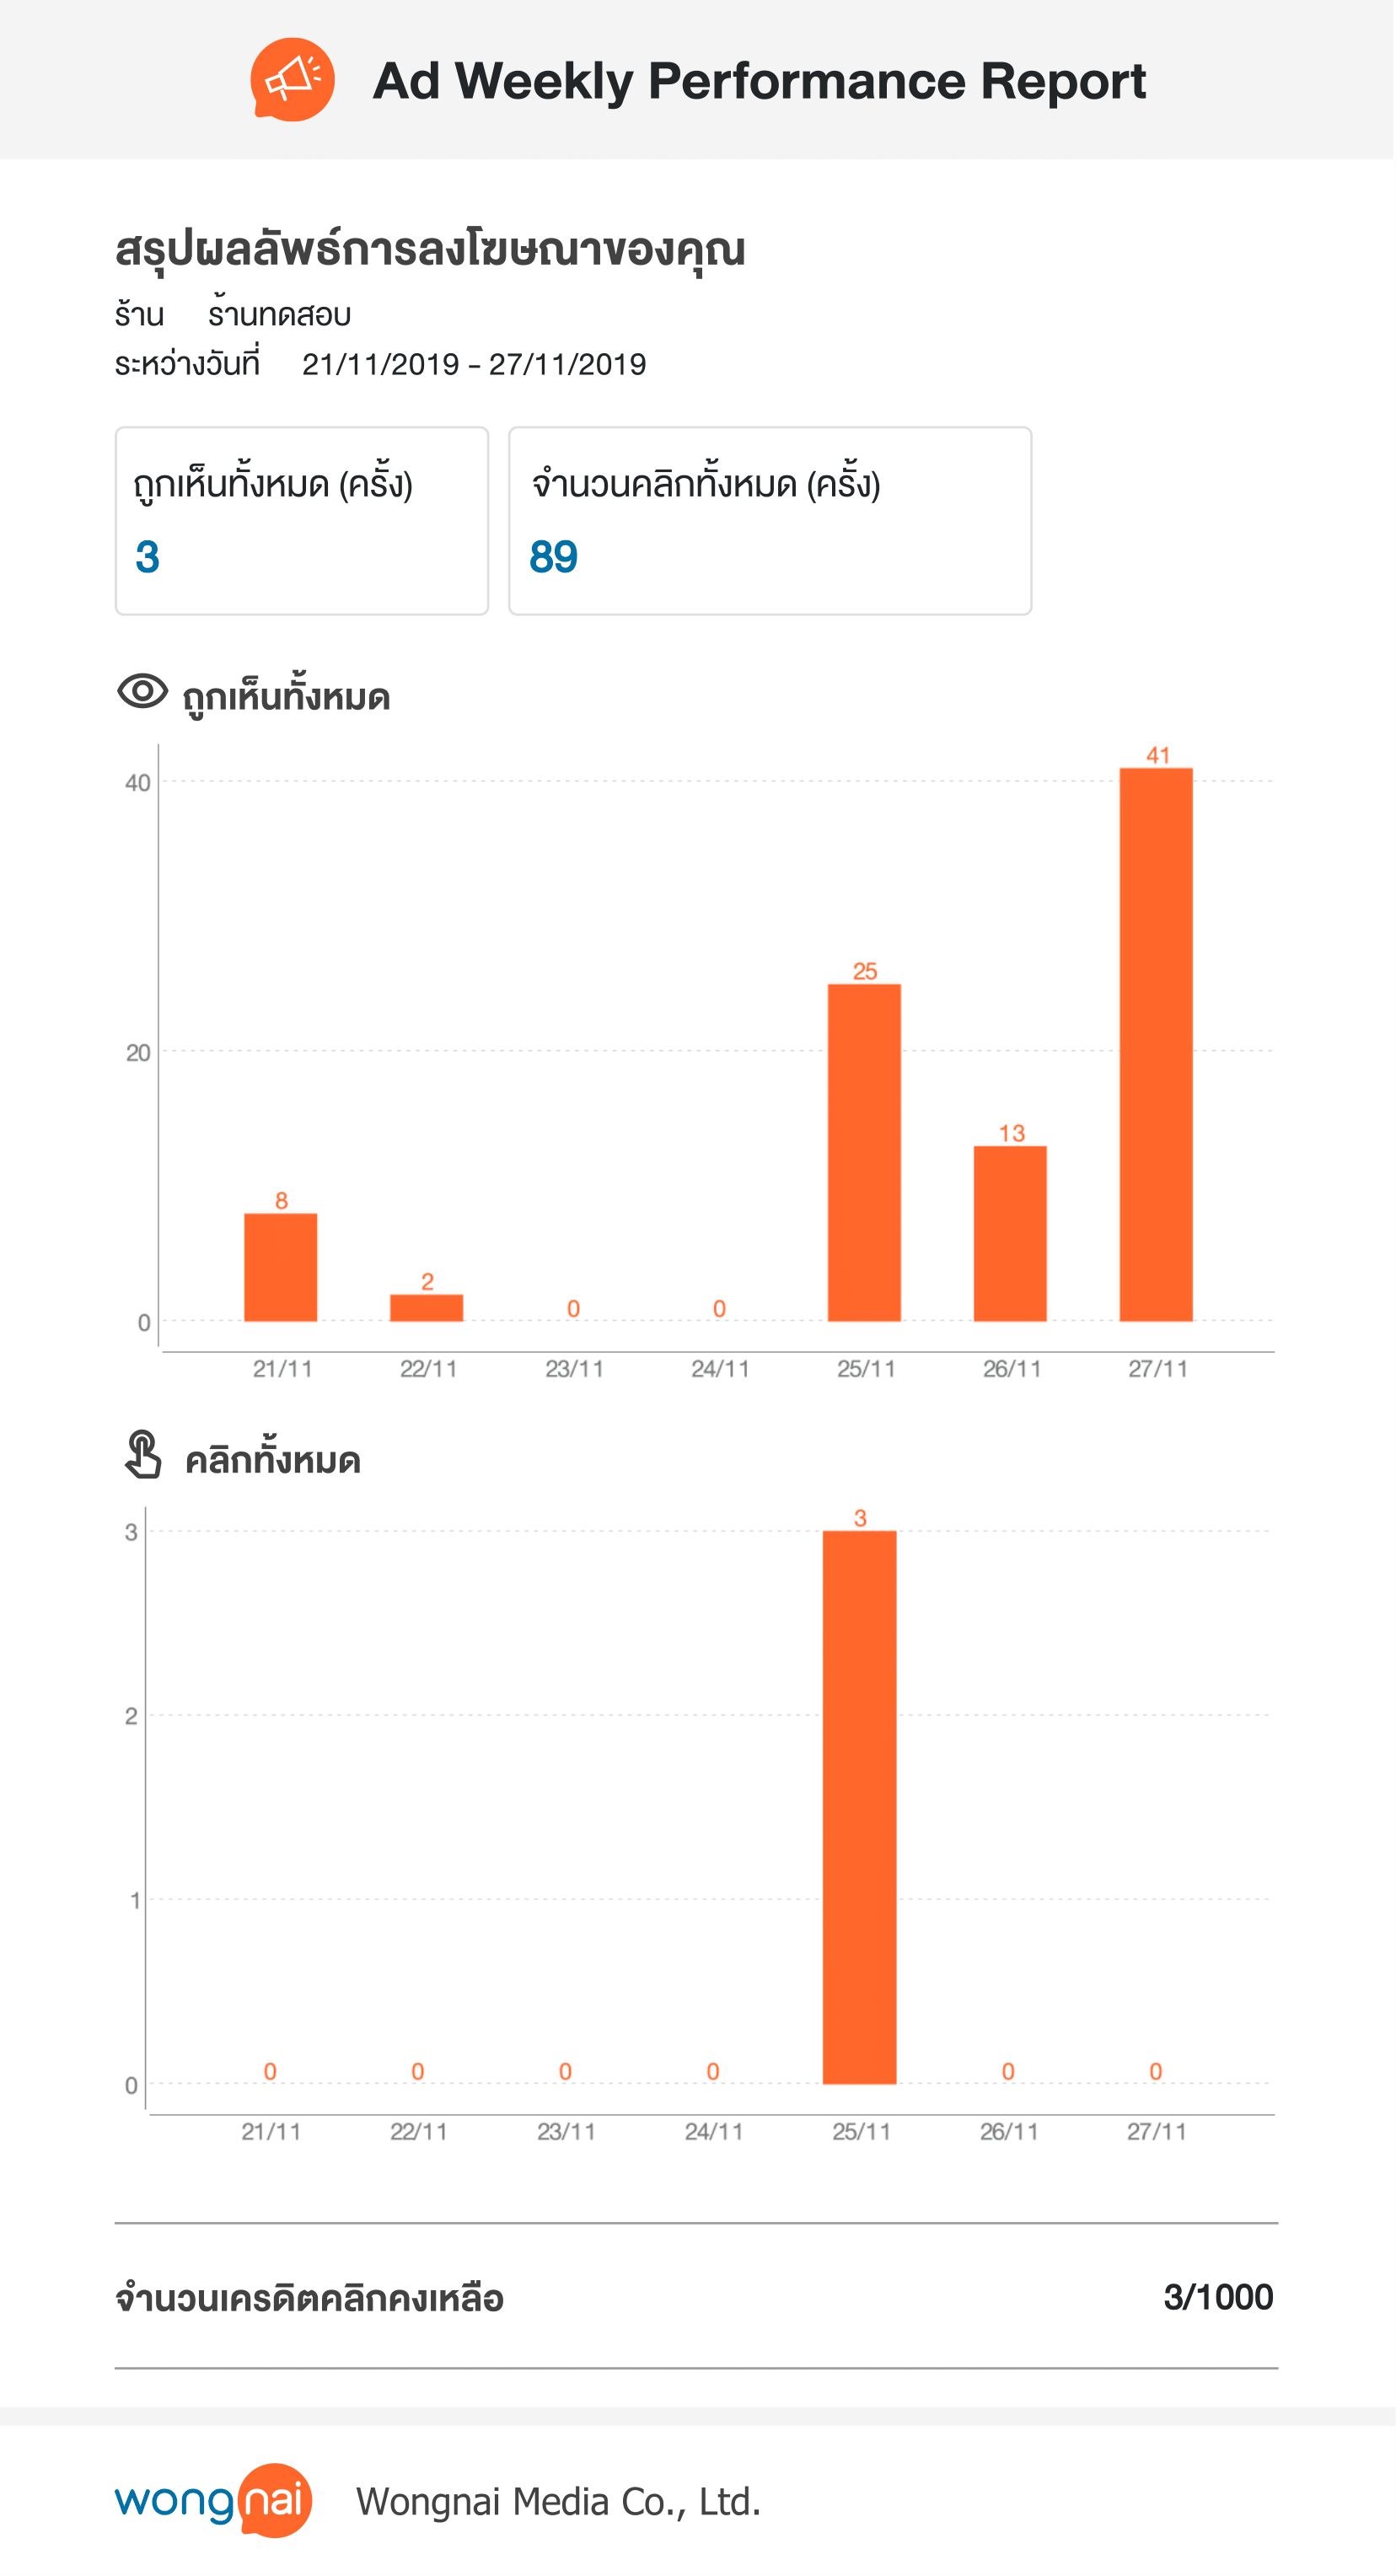
\includegraphics[width=0.9\textwidth]{report.png}  
	\caption{รายงานสถิติของโฆษณาที่ส่งให้ลูกค้า}
	\label{Fig:report}
\end{figure}
